\documentclass[../ESOF_notes.tex]{subfiles}

\begin{document}

\section{Basic Concepts}

Software Architecture is the fundamental organization of a system, embodied in its components, their relationships to each other and the environment, and the principles governing its design and evolution.

\subsection{Design Level}
\begin{itemize}
    \item High-level design or \textbf{architectural design}: partition the system into components.
    \item Detailed design (e.g., object-oriented design): partition each component into classes.
    \item Design of algorithms and data structures.
\end{itemize}

\subsection{Typical outputs}
"Requirements Capture - "Architectural Design (high-level design)" - "Detailed Design" | "Coding" | "Unit Testing" - "Integration and Testing"

\subsection{Architectural design notations}
\begin{itemize}
    \item Block diagrams
        
        \begin{center}            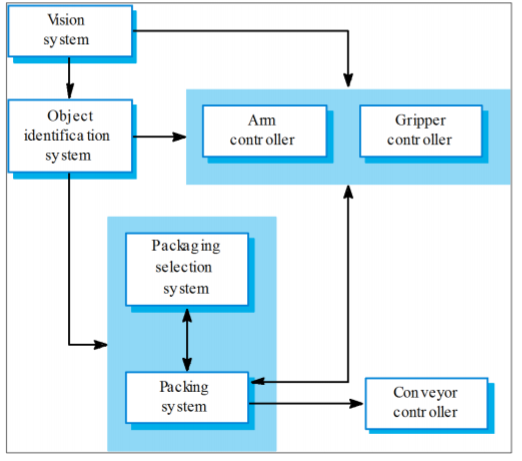
\includegraphics[width=8cm]{blockDiagrama.png}
        \end{center}
        \begin{itemize}
            \item Informal, but simple and easy to understand.
            \item The most frequently used for documenting software architectures.
            \item Lacks semantics and detail.
        \end{itemize}
        
    \item Architecture modeling languages (with UML)
        \begin{itemize}
            \item Semi-formal
            \item Multiple views
        \end{itemize}
    \item Formal architecture description languages (ADLs)
        \begin{itemize}
            \item Support automated analysis and simulation
        \end{itemize}
\end{itemize}

\subsection{Non-functional requirements}
Architectural design decision are strongly influenced by non-functional requirements:
\begin{itemize}
    \item Performance - Localize critical operations, minimize communications and levels of indirection
    \item Security - Use a layered architecture with critical assets in inner layers
    \item Safety - Localize safety-critical features in a small number of subsystems
    \item Availability - Include redundant components and mechanisms for fault tolerance
    \item Portability - Isolate platform dependencies in specific components
    \item Maintainability - Use fine-grained, loosely coupled, replaceable components.
\end{itemize}

\section{Architectural Views}

\subsection{Civil engineering analogy}
Architecture is best described by considering multiple views

\subsection{4+1 view model of software architecture}
    \begin{center}
        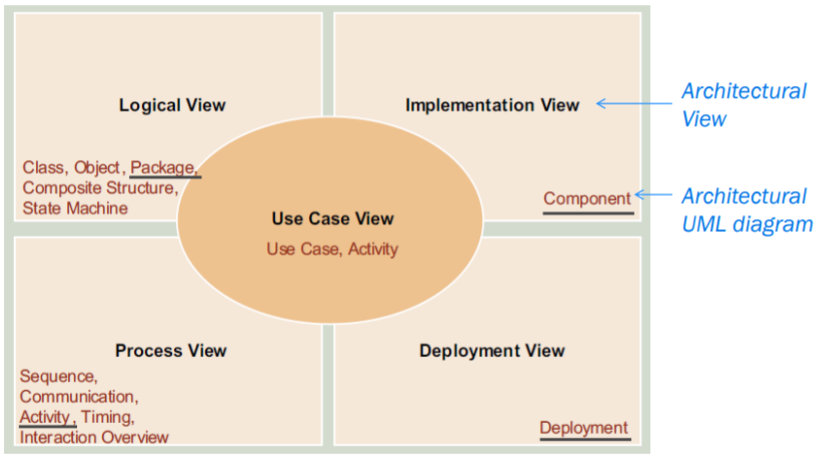
\includegraphics[width=12cm]{4-1-viewModel.png}
    \end{center}
    \begin{center}
        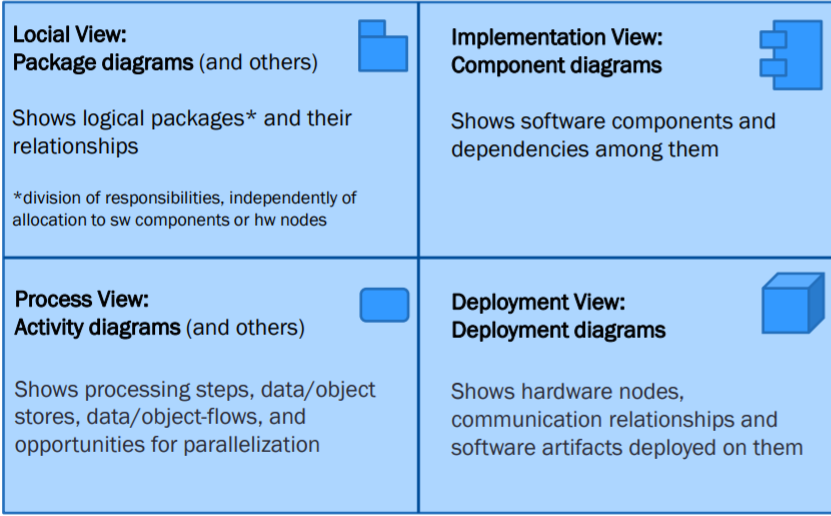
\includegraphics[width=12cm]{4-1-viewModel2.png}
    \end{center}
    \textbf{Use Case View (+1):} Relates the other views.

\section{Component Diagrams}
\begin{itemize}

    \item Components\newline A component represents a modular part of a system that encapsulates its contents and whose manifestation is replaceable within its environment.
    \begin{center}
        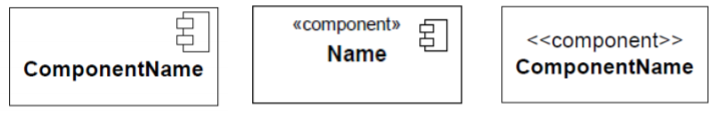
\includegraphics[width=10cm]{components.png}
    \end{center}
    
    \item Interfaces\newline A component defines its behavior in terms of \textbf{Interfaces provided (realized)} and \textbf{Interfaces required (used)}\newline Components with the same interfaces are interchangeable.
    \begin{center}
        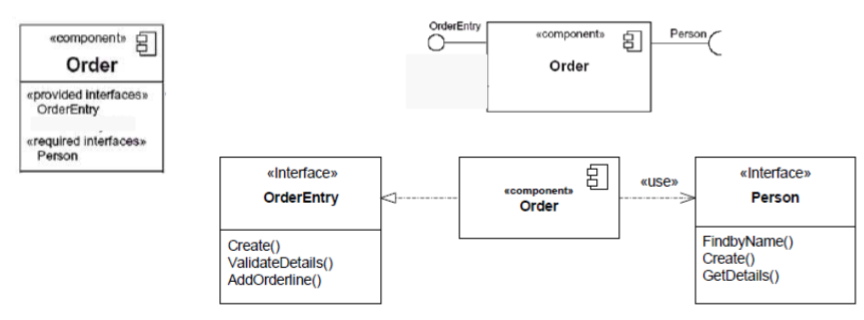
\includegraphics[width=10cm]{interfaces.png}
    \end{center}
    
    \item Dependencies\newline To promote intercangeability, components should not depend directly on other components but rather on interfaces (that are implemented by other components)
    \begin{center}
        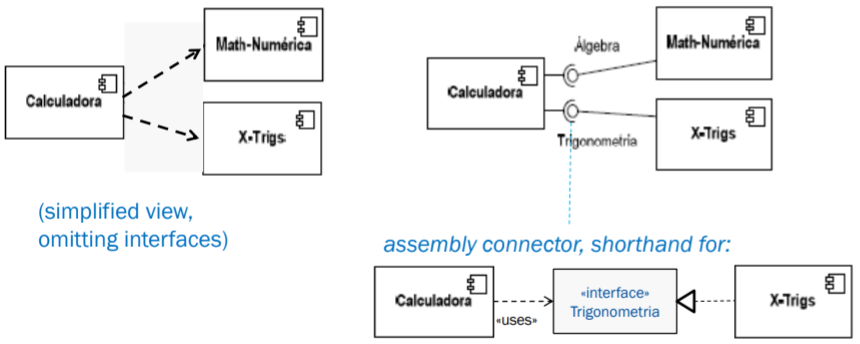
\includegraphics[width=10cm]{dependencies.png}
    \end{center}
    
    \item Components and classes\newline The behavior of a component is usually realized by its internal classes
    \begin{center}
        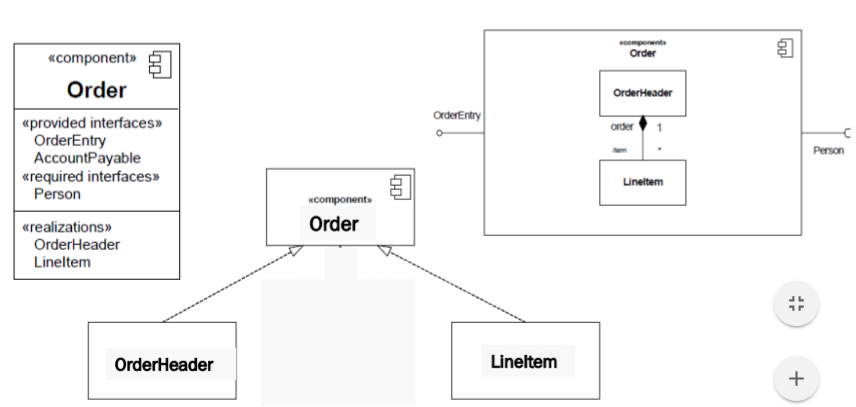
\includegraphics[width=10cm]{comp-classes.png}
    \end{center}
    
    \item Components and artifacts\newline Components manifest physically as artifacts (that may be deployed in hardware nodes)
    \begin{center}
        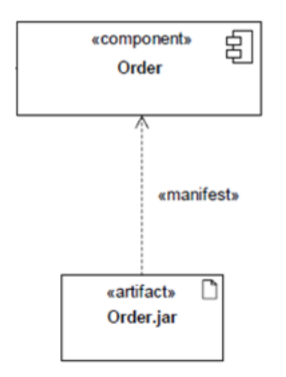
\includegraphics[width=5cm]{comp-artifacts.png}
    \end{center}
\end{itemize}

\section{Deployment Diagrams}
\begin{itemize}
    \item \textbf{Nodes}\newline Nodes are computational resources where artifacts may be deployed
    \item \textbf{Artifacts}\newline Artifacts are physical information elements used or procedure by a software development process. (example: model files, source code files, executable files, scripts, etc).
\end{itemize}

\section{Package Diagrams}
    \begin{center}
    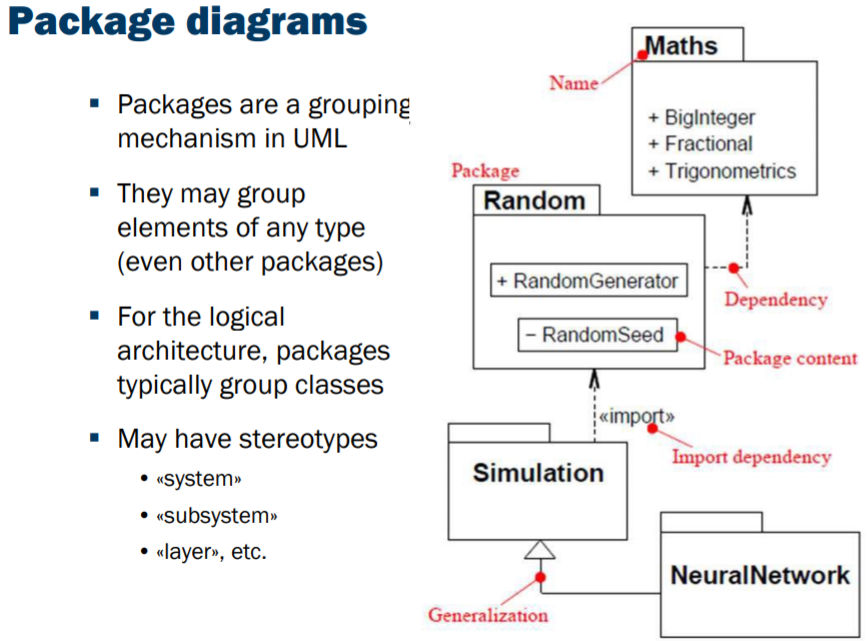
\includegraphics[width=10cm]{packageDiagrams.png}    
    \end{center}
    
\section{Activity Diagrams}
    \textbf{Compiler Architecture}
    \begin{center}
    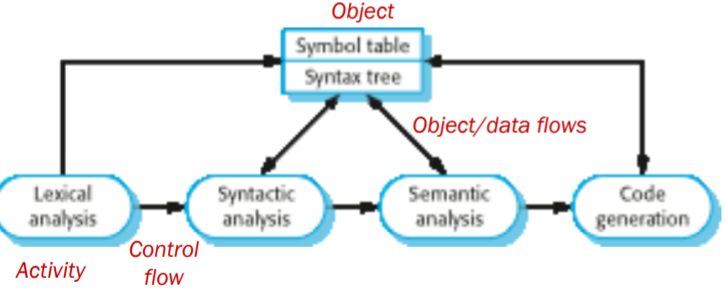
\includegraphics[width=10cm]{compilerArch.png}    
    \end{center}

\newpage

\section{Architecural Patterns}
    \begin{itemize}
        \item Patterns are a means commonly used in software engineering of representing, sharing and reusing knowledge.
        \item A pattern describes a proven solution for a recurring problem in a context "Pattern = (Context, Problem, Solution)"
        \item An architectural pattern (or architectural style) is a stylized description of good architectural design practice, which has been tried and tested in different environments.
    \end{itemize}
    
    \subsection{Mode-view-controller (MCV)}
    For interactive processing
    Separates presentation \textbf{(V)} and interaction \textbf{(C)} from the application data/sate \textbf{(M)}.\newline Example: Ruby on Rails.\newline\newline
        \textbf{When used:} 
        \begin{itemize}
            \item There are multiple ways to view and interact with data.
            \item Future requirements for interaction and data presentation are unknown.
        \end{itemize} \textbf{Advantages:} 
        \begin{itemize}
            \item Allows the data and its representation to change independently.
            \item Supports presentation of the same data in different ways.
            \item Changes made in one data representation are shown in all of them.
        \end{itemize}
        \textbf{Disavantages:}
        \begin{itemize}
            \item Code overhead for simple data model and interactions.
        \end{itemize}
        
    \subsection{Pipes and filters (data flow)} - For batch processing\newline\newline
        Organizes the system as a set of data processing components (filters), connected so that data flows between components for processing (as in a pipe).\newline Example: Compiler Architecture, Test Generation Tool.\newline\newline
        \textbf{When used:} 
        \begin{itemize}
            \item In data processing applications (both batch- and transaction based) where inputs are processed in separate stages to generate outputs.
        \end{itemize}
        \textbf{Advantages:} 
        \begin{itemize}
            \item Easy to understand and supports transformation reuse.
            \item Workflow style matches the structure of many business processes.
            \item Evolution by adding transformations is straightforward.
            \item Can be implemented as either a sequential or concurrent system.
        \end{itemize}
        \textbf{Disavantages:}
        \begin{itemize}
            \item Format for data transfer has to be agreed upon.
            \item Possible overhead in parsing/unparsing input/output data.
            \item Not really suitable for interactive systems
        \end{itemize}
        
    \subsection{Layered architecture}  For complex systems with functionalities at different levels of abstraction\newline\newline
        Organizes the system into a set of layers, each of which groups related functionality and provides services to the layer above. (Strict, Relaxed)\newline Example: Three-Layered Services Application, CASE Tool. \newline\newline
        \textbf{When used:} 
        \begin{itemize}
            \item When building new facilities on top of existing systems.
        \end{itemize}
        \textbf{Advantages:} 
        \begin{itemize}
            \item Supports the incremental development layer by layer.
            \item Lower layers provide isolation from system/platform specificities.
        \end{itemize}
        \textbf{Disavantages (strict layering):}
        \begin{itemize}
            \item Providing a clean separation between layers is often difficult and a high-level layer may have to interact directly with lower-level layers.
            \item Performance can be a problem because of multiple levels of interpretation of a service request as it is processed at each layer.
        \end{itemize}
        
        
     \subsection{Repositories (data centric)} 
     For accessing AND manipulating shared data by multiple subsystems\newline\newline
        All data in a system is managed in a central repository that is accessible to all system components or subsystems. Components or subsystems do not interact directly, only through the repository. (Variants: passive, active)\newline Example: IDE. \newline\newline
        \textbf{When used:} 
        \begin{itemize}
            \item In systems in which large volumes of information are generated that have to be shared and/or stored for a long time.
            \item In data-driven systems where the inclusion of data in the repository triggers an action or tool (active repository).
        \end{itemize}
        \textbf{Advantages:} 
        \begin{itemize}
            \item All data can be managed consistently as it is all in one place.
            \item Components can be independent (don’t need to know each other).
            \item Changes made by one component can be propagated to all others.
        \end{itemize}
        \textbf{Disavantages:}
        \begin{itemize}
            \item The repository is a single point of failure for the whole system.
            \item Possible inefficiency in having all communication through the repos.
            \item Distributing the repos. across several computers may be difficult.
        \end{itemize}
        
    \subsection{Client-server and n-tier systems}
    For accessing shared data and resources from multiple locations \newline \newline
    Asymmetrical distributed system in which clients request services from servers through a shared network or middleware.\newline N-tier systems are a generalization of client-server (2-tier) systems, in which servers may in turn act as clients. The tiers may also be implemented on a single computer.\newline Example: Film Library, Four-Tiered Web Application.\newline\newline
        \textbf{When used:} 
        \begin{itemize}
            \item When shared databases or other resources have to be accessed from a range of locations.
            \item Because servers can be replicated, may also be used when the load on a system is variable.
        \end{itemize}
        \textbf{Advantages:} 
        \begin{itemize}
            \item Servers can be distributed and replicated across a network.
            \item General functionality (e.g., printing) can be available to all clients. 
        \end{itemize}
        \textbf{Disavantages:}
        \begin{itemize}
            \item Each service is a single point of failure so susceptible to denial of service attacks or server failure.
            \item Performance may be unpredictable because it depends on the network as well as the system.
            \item Possible management problems if servers are owned by different organizations.
        \end{itemize}
    
    \subsection{Design models and design views}
    An object-oriented design model may in general cover 4 inter-related design views, represented by means of appropriate UML diagrams. \textbf{(External, Internal, Static, Dynamic)}
    
\section{Process stages}
    \begin{itemize}
        \item There are a variety of different object-oriented design processes that depend on the organization using the process.
        \item Common activities in these processes include:
        \begin{itemize}
            \item Define the system context and use cases;
            \item Design the system architecture;
            \item Identify the principal object classes in the system;
            \item Develop design models;
            \item Specify object interfaces (API).
        \end{itemize}
    \end{itemize}

\section{common use cases of UML sequence diagram in detailed design}
\begin{itemize}
    \item show interactions between the system and its environment
    \item show internal interactions between objects the system
    \item show a dynamic view of the system.
\end{itemize}
    
\section{Verification vs Validation}
    \begin{itemize}
        \item Verification – are we building the product right?
        \newline Ensure (mainly through reviews) that intermediate work products and the final product are “well built”, i.e., conform to their specifications
        \item Validation – are we building the right product?\newline
        Ensure (manly through tests) that the final product will fulfill its intended use in its intended environment\newline Can also be applied to intermediate work products, as predictors of how well the final product will satisfy user needs.
        \begin{center}            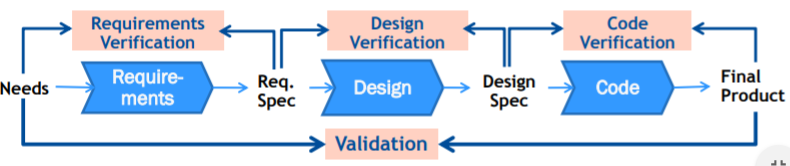
\includegraphics[width=10cm]{veriVSvali.png}
        \end{center}
    \end{itemize}
    
\section{Verification and validation technique}
    \begin{itemize}
        \item Static techniques – involve analyzing the static system representations to find problems and evaluate quality
        \begin{itemize}
            \item Reviews and inspections
            \item Automated static analysis (e.g., with lint)
            \item Formal verification (e.g., with Dafny)
        \end{itemize}
        \item Dynamic techniques – involve executing the system and observing its behavior
        \begin{itemize}
            \item Software testing
            \item Simulation (e.g., animation of state machine model)
        \end{itemize}
    \end{itemize}
    
\section{Software reviews and inspections}
    \begin{itemize}
        \item Analysis of static system representations to find problems
        \begin{itemize}
            \item Manual analysis of requirements specs, design specs, code, etc.
            \item May be supplemented by tool-based static analysis
        \end{itemize}
        \item Advantages (as compared to testing):
        \begin{itemize}
            \item Can be applied to any artefact, and not only code
            \item Can be applied earlier (thus reducing impact and cost of errors)
            \item Fault localization (debugging) is immediate
            \item Allows evaluating internal quality attributes (e.g., maintainability)
            \item Usually more efficient and effective than testing in finding security vulnerabilities and checking exception handling
            \item Very effective in finding multiple defects
            \item Peer reviews promote knowledge sharing
        \end{itemize}
    \end{itemize}
    
\section{Types of reviews}
    \begin{itemize}
        \item Process
        \begin{itemize}
            \item Personal review
            \item Walkthrough
            \item Peer review
            \item team inspection
        \end{itemize}
        \item Purpose
        \begin{itemize}
            \item Technical review
            \item Management review
        \end{itemize}   
        \item Target
        \begin{itemize}
            \item Requirements review/inspection
            \item Design review/inspection
            \item code review/inspection
            \item Reviewing plans and reports
        \end{itemize}   
    \end{itemize}
    
    \subsection{Review best practices}
    \begin{itemize}
        \item Use a checklist derived from historical defect data\newline Makes the review more effective and efficient, by focusing the attention on the most frequent and important problems.
        \item Take enough review time (e.g., 200 LOC/hour is a recommended review rate by some authors)
        \item Take a break between developing and reviewing (in personal reviews)
        \item Combine personal reviews with peer reviews or team inspections
        \item Measure the review process and use data to improve\newline size, time spent, defects found, defects escaped (found later).
    \end{itemize}
    
\section{Capture-recapture}
    The capture-recapture method is used to estimate the total defects (T) and number of defects remaining (R) based on the degree of overlapping between defects detected by different inspectors (A, B).

\section{Key points}
    \begin{itemize}
        \item Verification shows conformance with specification. Validation shows that the program meets the customer’s needs.
        \item Static verification techniques involve examination and analysis of the program for error detection. Dynamic techniques involve executing the program for error detection.
        \item Program reviews and inspections are very effective in discovering errors. 
        \item Source code in inspections is systematically checked by a small team to locate software faults.
    \end{itemize}

\section{Software Engineering Laws}

    \subsection{Lei Nº3 - Principio fundamental da Arquitetura de Software}
    Qualquer problema de estruturaçao de software resolve-se introduzindo niveis de indireção.\newline Corolário: Qualquer problema de desempenho resolve-se removendo niveis de indireção.
    
    \subsection{Lei nº4 - Lei de Arquimedes da Arquitetura de Software}
    Um sistema de software fundado numa má arquitectura afundar-se-á sob o peso do seu próprio sucesso.
    
\end{document}